\section{AlphaZero}
   
   We have looked at minimax, alphabeta pruning and MCTS. They all have nice theoretic guarantees and have been used in many applications. Their main limitation as previously mentioned with minimax is computation. MCTS on its own works fairly well in larger state spaces. There is a limit to this however and being able to solve a game as large as Go will require some modification to the algorithm. We saw how alphabeta pruning cuts out parts of the tree that we know are not adding any information to the decesion making process. Can we accomplish a similar thing with MCTS? The answer is yes, by utilizing deep learning. There have actually been many attempts to improve upon MCTS but fundamentally there are two ways to improve the search. You can either improve the depth of the search or the breadth of the search. In AlphaZero both depth and breadth are improved using neural networks. To give a quick visualization of this process look at the following three figures. They give a picture of a miniature game of Go. You start with an extremely large state space which can be seen in the first figure. You can imagine how large this picture would be if attempting to visualize the entire state space of the full game of Go or Chess. 
   
   \begin{figure}[h!]
       \centering
       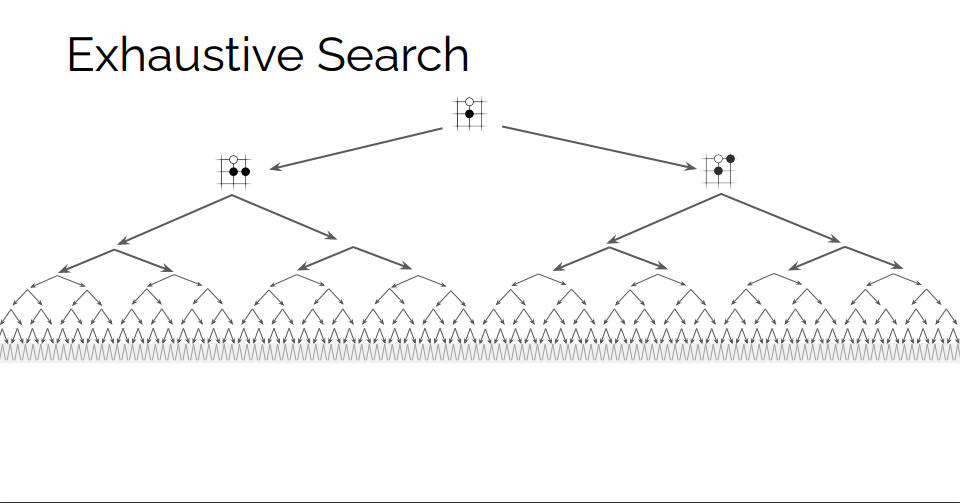
\includegraphics[width=300px,height=200px]{images/julian_exhaustive_search.png}
       \caption{Mini game of go}
       \label{fig:my_label}
   \end{figure}

    \begin{figure}[h!]
       \centering
       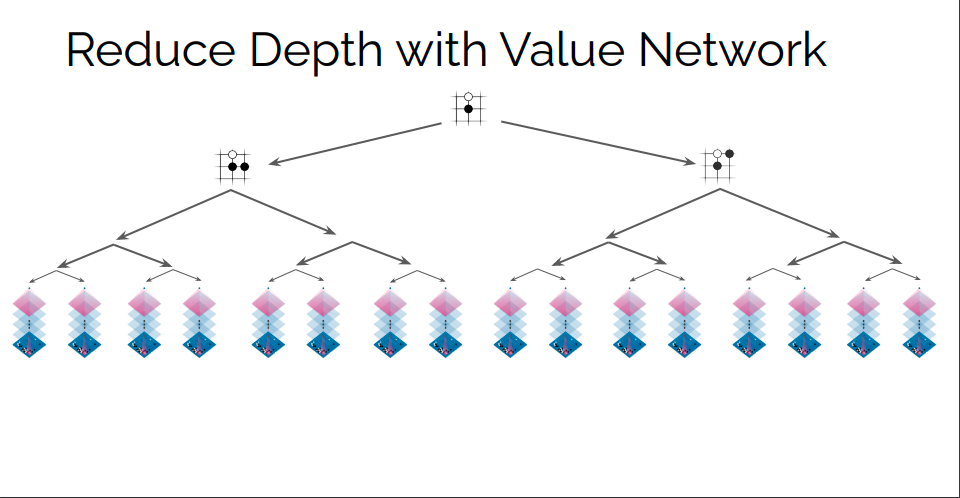
\includegraphics[width=300px,height=200px]{images/julian_reduce_value_network.png}
       \caption{Reduce depth}
       \label{fig:my_label}
   \end{figure}

    \begin{figure}[h!]
       \centering
       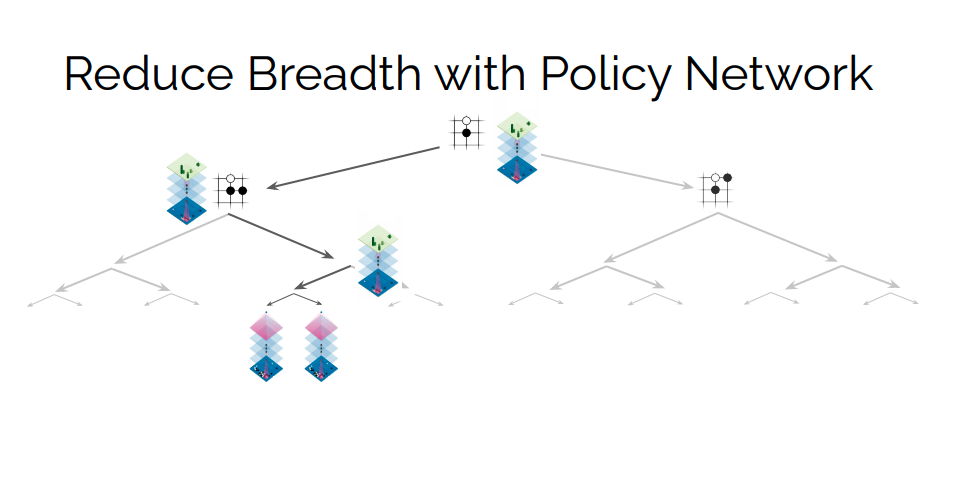
\includegraphics[width=300px,height=200px]{images/julian_reduce_policy_network.png}
       \caption{Reduce breadth}
       \label{fig:my_label}
   \end{figure}
   
   You can see that we have two neural networks a value network and a policy network. The value network (figure 4.2) and the policy network (figure 4.3) work in unison to reduce the state space to something more manageable. The obvious question is how do we actually go about learning both of these networks? 
   
   \section{Expert Data}
   
   Lets first start by actually defining what a value network and a policy network are. First recall that we define the value of a given state as $ v_{\pi}(s) = E_{\pi}[G_{t}| S_{t} = s]$ In the context of a game like Go there are two possible outcomes $ z= \{-1,1\}$. -1 for a loss and +1 for a win. So we can translate the value at a given state to mean a prediction of the outcome $z$ from a given state $s$. A value network is a neural network with weights $ \theta $ s.t. $ v(s,\theta) \approx v_{\pi}(s)$. A policy network on the other hand is a network that helps us with the task of mapping states to actions. Given network weights $\theta$ we have $\pi(a | s, \theta) = Pr\{A_{t} = a | s_{t} = s, \theta_{t} = \theta\}$. So the policy $ \pi $ is actually a distribution over actions. This policy will give you a probability of taking an action from a given state or board position. So this means our policy is stochastic it does not give us a single action to take. 
   
   The approach first introduced by deepmind [2] made use of expert data. We will not go into detail here about their approach but I want to highlight at least the intention of that paper. Assume we have an perfect oracle. That is we have some function $ f(s) \rightarrow v$  that can tell us the true value of being at any possible state? Then we are almost done and can happily do a single pass through the search space to obtain optimal path. At each node starting from the root node of the tree we just take the action that gives us the highest value. We can use our oracle for this by looking at each possible action and seeing which one leads to a state with a higher value. Typically we would have to know something about our opponents policy but here we can plan by acting as both players. We can just assume that our opponent has access to the same oracle and will play perfectly. 
   This can be summed up with the following bellman equation.
   $ a = \underset{a}{argmax} \sum_{s^{'},r} p(s^{'},r | s,a) [r + \gamma f(s^{'})]$. This equation is a form of the bellman optimally equation. Lets break down each part. We are interested in finding the action that gives us the highest return. $ \sum_{s^{'},r} p(s^{'},r | s,a) $ simply means that we are going to look at each of the possible next states assuming we have taken a specific action from our starting state s. This will gives us a probability of each one of those states which we will use to weight the second part of the equation by. The second part $[r + \gamma f(s^{'})]$ is the return that we expect to get
    This assumes you have knowledge of the environment (i.e. you can compute $p(s^{'},r | s,a) $ ). This is an assumption made by MCTS and by the AlphaGo algorithms.
    Since we dont have an oracle we can start thinking about other ways to approximate $f(s)$. Most ways that have been tried historically are taking advantage of expert knowledge. This can be in the form of explicitly hard coding a way to evaluate the value of a state. This has been done in games as complex as chess. You might do something naive like assign a value to each piece. Then count up all the pieces that each side has and assign them a score. 
    
    You could do as more advanced chess programs did and create a database of positions with the actions that were taken by experts at each position. Then you could create a lookup table or another way to approximate a good policy function $ \pi^{*}(s) \rightarrow a $. This second approach is what the first version of AlphaGo did and we will now look at this more deeply. 
    Assume we have created a database of expert games (or other environments). So we have an unordered list of tuples of positions,actions and outcomes. that were played during actual games. That is we have $ (s_{0}, a_{0}, z_{0}), (s_{1}, a_{1}, z_{1}), (s_{2}, a_{2}, z_{2}),..... (s_{n}, a_{n}, z_{n}) = \textbf{D}$ where $s \epsilon \mathbb{R}^{d} , a \epsilon \mathbb{R}^{|A|}$ and as stated before $ z= \{-1,1\}$. There are \textit{n} samples in our database, each state is a vector of size \textit{d} and each action is of size $|A|$ the possible number of actions. We will assume for convenience that d is the dimensions of the environment. If we were playing chess than the board could be represented by a vector of size 8 x 8 = 64. So the set of legal actions will be something $ \leq 64 $ but the state will most likely be $
    \geq d $. For instance we will see that Deepmind used something $ > d$ to represent state. 
     We can sample from the expert $ (s,a) \sim \mathbf{E} $ where $ s $ is some state and $a$ is the action taken by the expert in that state. Sampling from $\mathbb{E}$ will be done uniform randomly s.t. there is no correlation from one sample to the next to help avoid over fitting concerns. 
    We can then employ any of a number of Supervised Learning techniques to learn a policy function $ \hat{f}:s \rightarrow a$ by sampling a large number of data points from $\mathbf{E}$ and minimizing some loss function $L(\hat{f}, \mathbf{E})$. We can do a similar thing to learn a value function by sampling state outcome pairs from the database as well$ (s,z) \sim \mathbf{E} $. The loss function used for the policy network is cross entropy loss and for the value network it is mean squared error. For AlphaGo Fan the first AlphaGo algorithm this was just the seeding step. Once you have your expert networks than you use self-play and MCTS to further improve upon them. There are many details that go into AlphaGo Fan and I encourage the reader to go read the paper if interested [2]. The main thing I want us to think about here is that we are able to use generated data to reduce the depth and breadth of our search. Recall that in MCTS we select actions by 
    
    \begin{equation}
      a = \underset{a}{argmax}(Q(s,a) + U(s,a))
    \end{equation}
    
    In AlphaGo Fan the breadth of the MCTS is reduced by using the policy network to help estimate the uncertainty term U(s,a). 
    
    \begin{equation}
        U(s,a) \propto \frac{P(s,a)}{(1 + N(s,a))}
    \end{equation}
    
    Where P(s,a) comes from the policy network. Reducing the depth is done by replacing the rollout step in MCTS by a rollout network trained on the expert data as well as a value network to help in estimating Q(s,a)
    
    \begin{equation}
        Q(s,a) \propto v(s,\theta)
    \end{equation}
    
    AlphaGo Zero actually makes the architecture much simpler. We will now turn to looking at that and again the reader if interested is encouraged to look at [2] for a more thorough reading of AlphaGo Fan. 
    
    \section{Zero Knowledge}
    
    I first want to highlight some of the main differences between AlphaZero and past implementation like AlphaGo Fan. 
    \begin{itemize}
         \item AlphaGo Zero is trained through self-play only. Starting from random play. There is no expert data used whatsoever. 
         
         \item The input features are only the black and white stones from the board. 
         
         \item It uses a single neural network to represent both the policy and values network. 
         \item It uses a simpler tree search that relies on the single network. It manages to avoid the need for rollouts. 
     
    \end{itemize}

      A big change in accomplishing the above was to move the lookhead search inside the training loop. In AlphaGo Fan the networks were trained first and then those networks were used to run MCTS. In AlphaGo Zero we will see that the network is trained during MCTS. 
    
    The network in short takes in the current board representation and history and outputs a vector of move probabilities and a value.  $ (p,v) = f_{\theta} (s) $. p gives the probability distribution of selecting action a in state s. $ p_{a} = Pr(a|s) $ 
    
    The below diagram gives a nice summary of the training pipeline. Lets look at part $\textbf{a}$ and $\textbf{b}$ separately. 
    
    \begin{figure}[H]
       \centering
       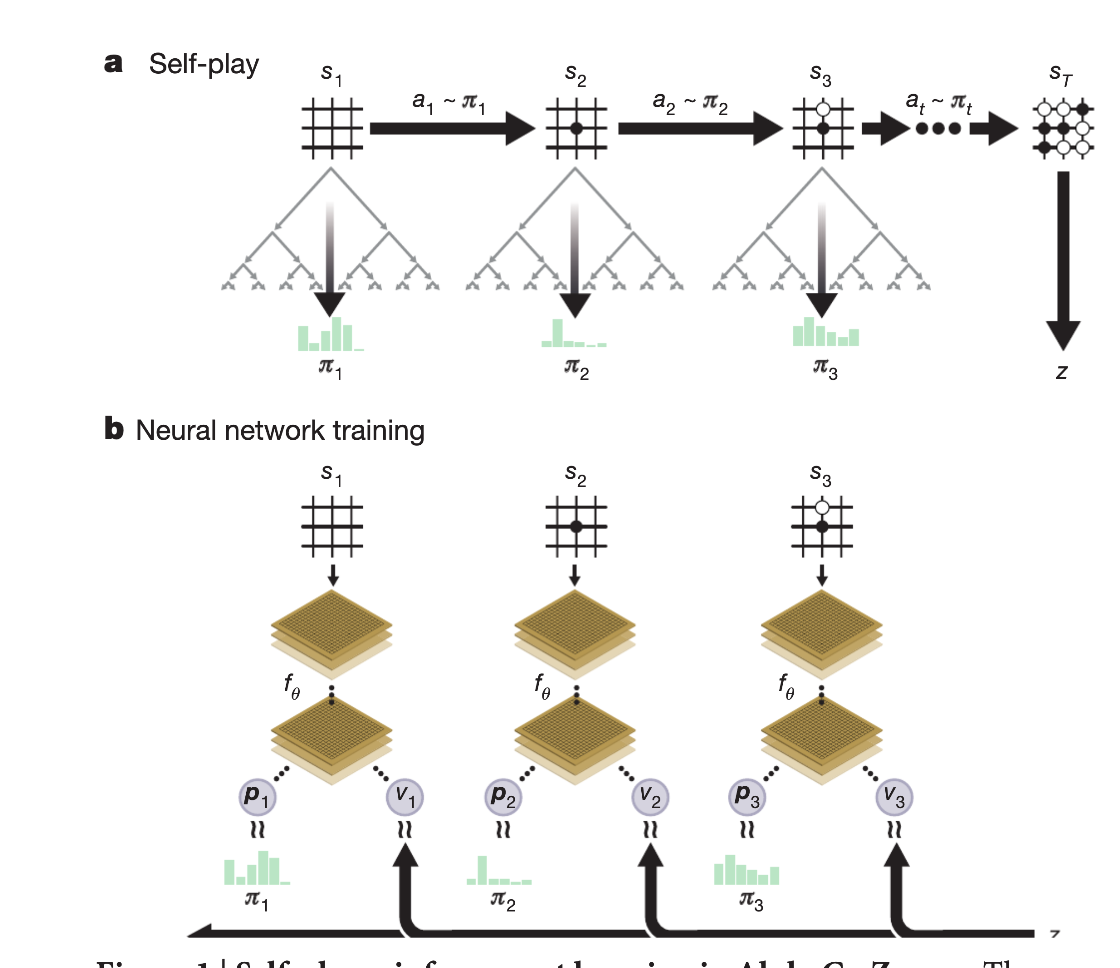
\includegraphics[width=300px,height=150px]{images/alpha_paper_figure_1.png}
       \caption{AlphaZero training pipeline}
       \label{fig:my_label}
   \end{figure}
    
    \textbf{a. Self-play} For each state $s_{t}$ in an episode (game) MCTS is performed and an action is sampled from the move probabilities it outputs. So we can think of MCTS as a function $ \alpha_{\theta} (s_{t}) \rightarrow \pi_{t}$ that takes in the current state and outputs the policy at that point in time. An action is than selected $a_{t} \sim \pi_{t} $ and executed against the environment. We repeat this process until we reach a terminal state and the game ends. We receive a reward from the environment $r_{T} \in (-1,1)$ which we can than use to train the network. 
    
    \textbf{b. Neural Network Training} From part $\textbf{a}$ we have a series of states and outcomes that we can use to improve the network. A single iteration of MCST gives us a series of data points like the following $(s_{1},\pi_{1},z_{1}),(s_{2},\pi_{2},z_{2}),......(s_{T},\pi_{T},z_{T})$ where $z_{t} = \pm r_{T}$. We can now use these to train the network. We will get into the details of the network architecture later but for now it will suffice to know that the loss function is minimized used SGD with the following loss $ l = (z - v)^{2} - \pi^{T} \log p + c ||\theta ||^{2} $. So the loss has three parts. MSE between the networks value prediction and the true outcome, a cross-entropy loss between the distribution output by MCTS and the distribution given by the network, and L2 weight regularization. 
    
    This process can be viewed as an attempt to make the network more closely resemble the outcome that is being given by MCTS. In this way MCTS acts as the guide for continual improvement. The search probabilities $\pi$ are generally going to give better action selections than what the current network advises. So MCTS acts as policy improvement operator. Also the outcome of games $\textbf{z}$ were obtained using MCTS and so they can be viewed as a policy evaluation operator. If you have a way to both improve a policy and evaluate the new policy than you have a way to perform policy iteration.
    
    Ok now we will dig into the MCTS a bit more and then take a look at how the network is trained after that. The below diagram taken from the paper displays each of the steps. Lets go through each
    
    \begin{figure}[H]
       \centering
       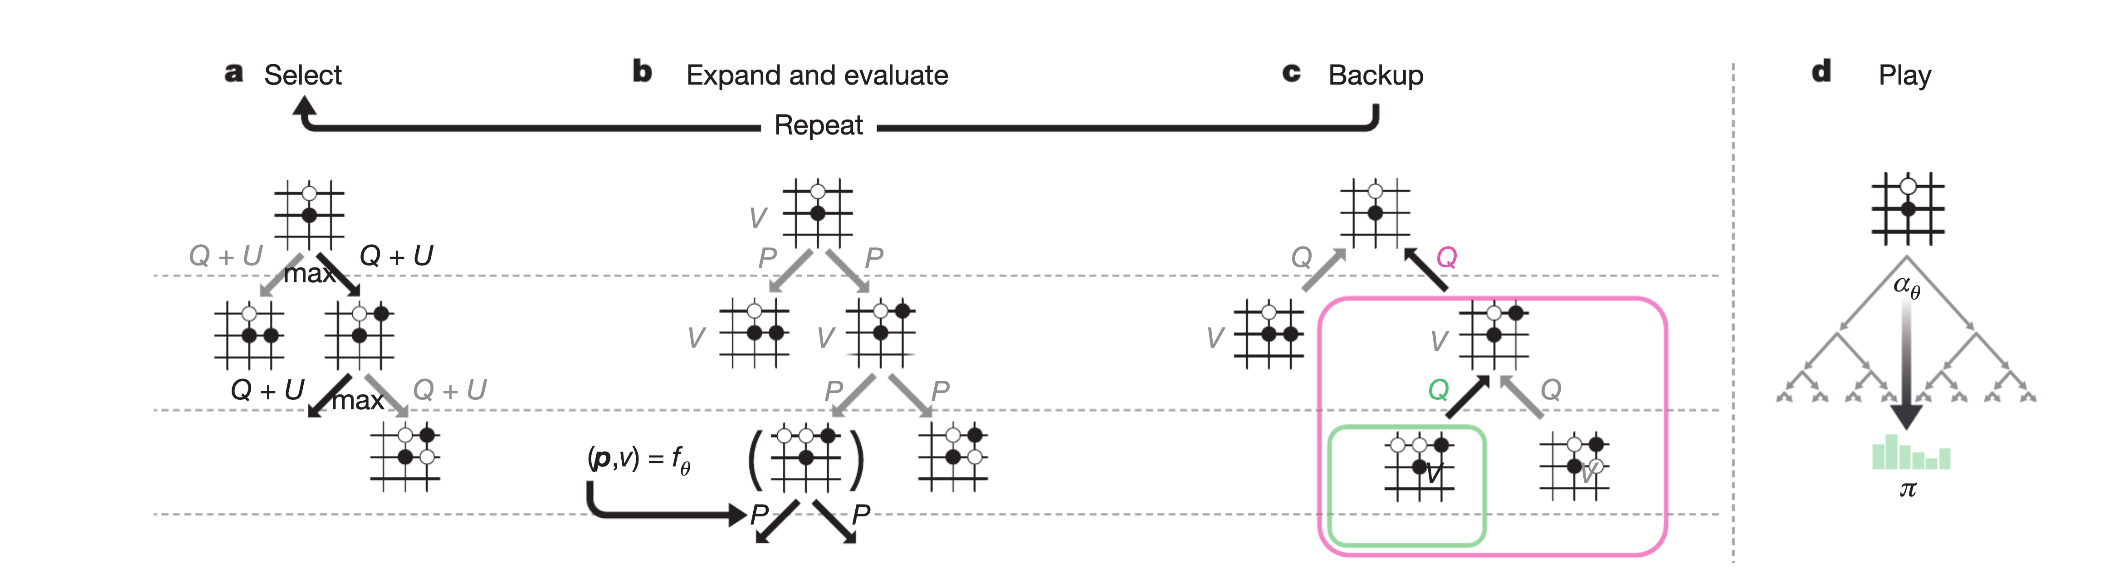
\includegraphics[width=300px,height=150px]{images/alpha_paper_figure_2.png}
       \caption{AlphaZero training pipeline}
       \label{fig:my_label}
   \end{figure}
   
   \textbf{Overview} Each \textbf{edge} in the tree stores a set of statistics. For all legal actions from a given node $ a \in A(s) $ the set $\{ N(s,a),W(s,a),Q(s,a),P(s,a) \}$ is stored. $N(s,a)$ is the visit count, $W(s,a)$ it the total action-value, $Q(s,a)$ is the mean action value, and $P(s,a)$ is the prior probability given by the network for the (s,a) edge. 
       
   The algorithm starts at the root node of the tree and then repeats steps (a-c) a given number of times. After these simulations are complete an action is selected based off of the accumulated statistics. The current node of the tree is moved to the next node based off of the action that was selected. The process is repeated for the new node until a terminal node is reached. The results are stored in order to train the network and the process is repeated from the root node once again. 
   
   \textbf{Selection} As with all the versions of MCTS we have looked at so far selections are made by taking actions by taking the max of a value term plus an upper confidence bound term. $\underset{a}{argmax} (Q(s,a) + U(s,a))$ In this case both terms come from the network. $U(s,a) \propto P(s,a) / (1 + N(s,a)) $ where $P(s,a) $ is given by the probability distribution over action $\textbf{p}$ from the network. $Q(s,a) = \frac{1}{N(s,a)}\sum_{s^{'}|s,a \rightarrow s^{'}}V(s^{'})$ So $Q(s,a)$ is just the mean over the value of the next states
   
   \textbf{Expand and evaluate} Once a leaf node is reached the leaf node is expanded and the leaf node is evaluated by the neural network. $ (P(s_{L}),V(s_{L})) = f_{\theta}(s) $ Then each edge is initialized with the following $\{ N(s,a) = 0,W(s,a) = 0,Q(s,a) = 0,P(s,a) = p_{a} \}$. The value of the leaf node $\textbb{v}$ is backed up. 
   
   \textbf{Backup} For each step that was visited from step (a,b) the statistics for each of the visited edges are updated. $N(s_{t},a_{t}) += 1$ , $W(s_{t},a_{t}) += \textbb{v} $, and $Q(s_{t},a_{t}) = \frac{(s_{t},a_{t})}{N(s_{t},a_{t})} $
   
   \textbf{Play} After a given number of iterations from the current node an action is selected and executed against the environment. The policy that is output by MCTS is given by the following formula. $\pi(a|s) = \frac{N(s,a)^{\frac{1}{\tau}}}{\sum_{b}N(s,b)^{\frac{1}{\tau}}}$
       
   $\tau$ is called a temperature parameter that controls the level of exploration. For each time step the statistics in the tree below the node of interest are retained. The statistics above are discarded and will be repopulated in the future if that node is revisited.
   
   We will now turn to focusing on the deep learning aspect of the algorithm. We have already discussed how data is collected and what loss function is used while training. Lets start with what the input looked like and than look at the architecture of the network itself. The input to the NN is a 19x19x17 image stack. There are 8 images for the current player and 8 for opponent and The final layer being a representation of who is to play. So the feature input at time $t$ is $s_{t} = [X_{t},Y_{t},X_{t - 1},Y_{t -1},... X_{t-7},Y_{t-7},C]$. Here $X_{t}$ is a 19 x 19 frame of ones and zeros. The ones representing the position of all of blacks stones at time t. Likewise $Y_{t}$ is the same except all ones for whites stones and zero elsewhere. C here is a 19 x 19 frame representing the player to act at time $t$. Its a frame of all ones if it is black to act and all zeros if it is white to act. 
   
   As mentioned previously the network used in AlphaZero is a two headed network. There is a single convolutional layer that processes the input followed by 39 residual blocks. Then the policy head consists of a convolutional layer, batch norm, relu and a fully connected layer. The value head is similar but with an extra convolutional layer and the output contains a $tanh$ function which works well for two player games since that constrains values to be between -1 and 1. They found that residual blocks performed better than convolutional layers. I think for understanding the core concepts it is not necessary to fully understand how all of the pieces of the deep learning architecture work. In the next section we will look at what it takes to build a smaller example of the architecture on your own. We will also look at some experiments that I ran using the game of ticatactoe and connect4 to help clarify some of the concepts discussed so far. 
    